\documentclass{article}
\usepackage[utf8]{inputenc}
\usepackage{graphicx} 

\begin{document}

Organizator počinje proces kreiranja novog zadatka slanjem zahtjeva web-aplikaciji.
Web-aplikacija provjerava da li je korisnik s pravima voditelja natjecanja.

\textbf{Ako je korisnik voditelj natjecanja:}
\begin{itemize}
  \item Web-aplikacija omogućuje pristup formi za unos zadatka.
  \item Organizator unosi detalje zadatka i testne primjere te šalje podatke.
  \item Web-aplikacija sprema zadatak u bazu podataka.
  \item Web-aplikacija šalje potvrdu organizatoru o uspješnom kreiranju zadatka.
\end{itemize}

\textbf{Ako korisnik nije voditelj natjecanja:}
\begin{itemize}
  \item Web-aplikacija šalje poruku organizatoru da samo voditelj natjecanja može kreirati zadatke.
\end{itemize}

\begin{figure}[h!]
  \centering
  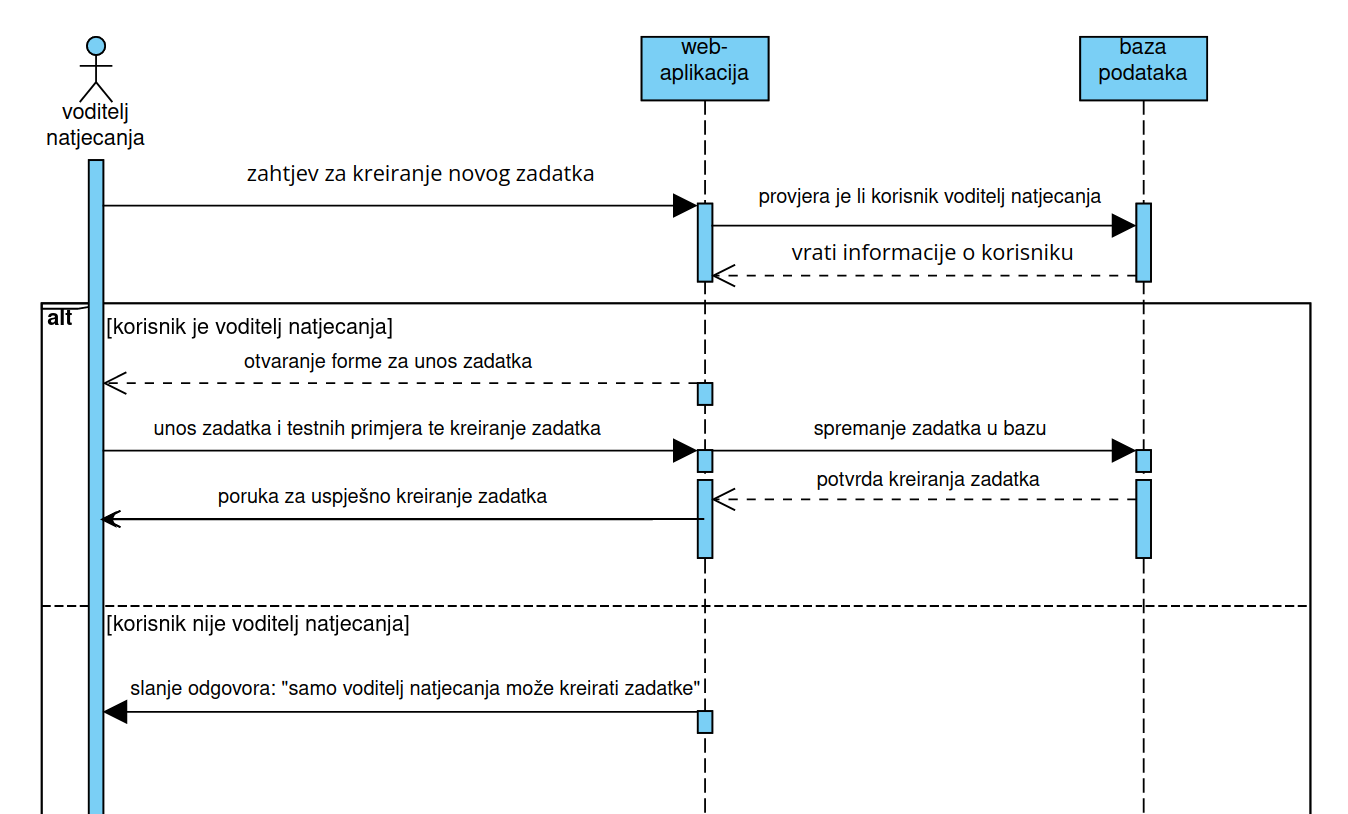
\includegraphics[width=\linewidth]{../slike/kreiranje_zadatka.png}
  \caption{Sekvencijski dijagram kreiranja zadatka}\label{fig:taskcreationdiag}
\end{figure}

\end{document}
